\documentclass[a4paper,leqno]{article}

\usepackage[T1]{fontenc}
\usepackage[utf8]{inputenc}
\usepackage[english]{babel}
\usepackage{amsmath}
\usepackage{longtable} 
\usepackage{multirow} 
\usepackage{graphicx}
\usepackage{algorithm2e}
\usepackage{listings}

\begin{document}
	
	
	\date{2017/11/26}
	\author{Bolshakova Liubov\\ Campagnoli Chiara\\ Lagni Luca}
	\title{\textbf{\huge Travlendar+}\\ Design Document}
	\begin{minipage}[!t]{\linewidth}
		\centering
		
\includegraphics[scale=0.8]{logo2}
	\end{minipage}
	\begin{minipage}[!h]{\linewidth}
		\maketitle 
	\end{minipage}
	
	\newpage
	\tableofcontents                        
  
\newpage	
\section{Introduction}

\subsection{Purpose}
The purpose of this document is to provide information about the design decisions we made for the development of the system Travlendar+. More in detail, it includes an overview about architectural design, description and interactions of the main components of the system, some possible design patterns that can be used for implementation, the description of some of the main algorithms and the plan of implementation, integration and test. It is mainly addressed to the developers of the system.

\subsection{Scope}
Travlendar+ is a calendar based applications, which allows the user to create meetings with different locations and computes the best way to reach such locations. It includes different means of tansport, both public and personal, autonomous and not. Amonng its functionalities there are the possibility of creating flexible breaks between meetings, deselecting travel means the user does not wish to use and choosing the combination of travel means which minimizes the carbon footprint. Besides, it supports the user in the reservation of cars and bikes of a vehicle-sharing service and in the purchase of tickets of public transport companies.\\
More details about the goals and functionalities of the system can be found in the RASD.

\subsection{Definitions, Acronyms, Abbreviations}
\begin{itemize}
	\item API: Application Programming Interface.
	\item DD: Design Document
	\item GPS: Global Positioning System.
	\item GSM: Global System for Mobile Communications.
	\item GUI: Graphical User Interface.
	\item OAMOT: Other Autonomous Means of Transport
	\item ONAMOT: Other Non-Autonomous Means of Transport
	\item OS: Operating System.
	\item RAM: Random-access memory.
	\item RASD: Requirement analysis and Specification Document.
	\item SMS: Short Message Service.
\end{itemize}

%\subsection{Revision history}

\subsection{Reference Documents}
\begin{itemize}
	\item Mandatory Project Assignments.pdf
	\item Requirements Analysis and Specification Document
	\item Design Deliverable Sample from A.Y. 2015-2016.pdf
	\item DD From the car sharing project.pdf
	\item Integration and test plan from the car sharing project.pdf
\end{itemize}

\subsection{Document Structure}
Besides the introduction, the document is divided into five main parts:
\begin{enumerate}
	\item Architectural design: it contains all the main decisions about the general architecture of the system. In particular, here is specified the tier division of the proposed system and are included the main diagrams (component diagrams, deployment diagrams, runtime diagrams and the complete class diagram). Here are also described some of the possible design patterns which can be used for implementation.
	\item Algorithm design: it includes a description of some of the main algorithms that will be used to implement our system.
	\item User interface design: it inludes some mockups of the mobile application interface, undelying how the main functionalities of the system can be accessed by the user.
	\item Requirements traceability: it explains how the requirements identified in the RASD have been fullfilled in the design elements and decisions.
	\item Implementation, integration and test plan: it explains the order in which we are going to implement, integrate and test the components of the system.
\end{enumerate}

\newpage
\section{Architectural design}

\subsection{Overview}
Travlendar+ is based on a three-tier architecture. A diagram of the proposed system was already present in section 2.4.3 of the RASD; here we provide on the same diagram a division between the different tiers and a more detailed description of each one of these.

\begin{figure}[!h]
	\begin{centering}
		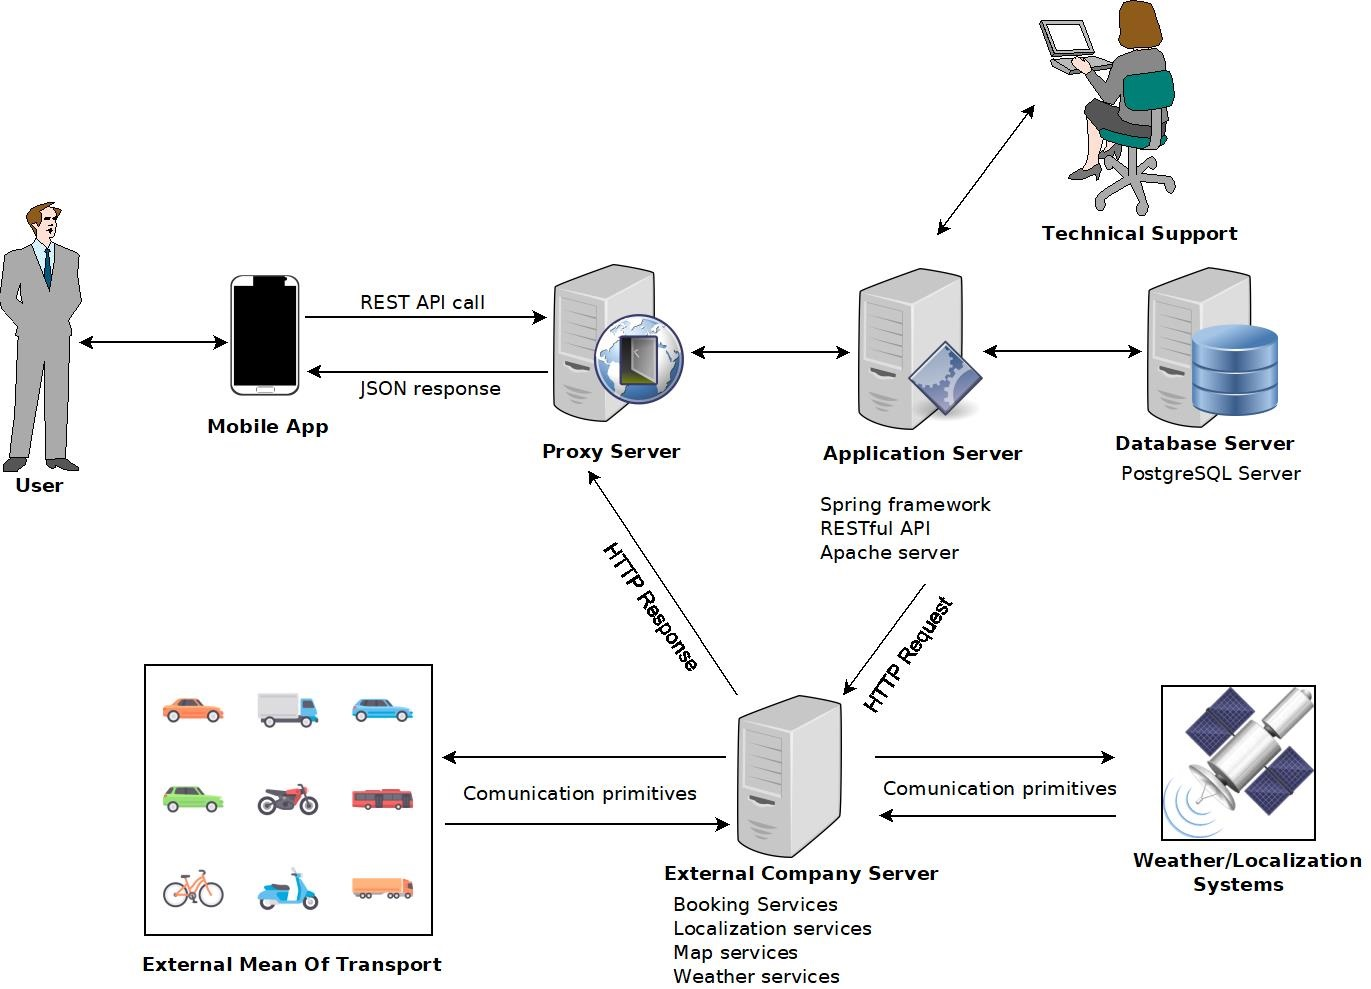
\includegraphics[scale=0.3]{ProposedSystemDiagram_29102017_1}
	\end{centering}
	\caption{Proposed system with tier division. Red: presentation, Blue: logic, Green: data}
\end{figure}

The presentation layer consists of the mobile application, which provides a GUI for the interaction of the user with the service.\\
The logic layer is mainly represented by the application server, where all main decisions and computation take place, although a small part of logic is left to the mobile application (simple elaborations of data such as the location of the user through GPS, or remodeling of the view presented to the user).\\
A proxy server is inserted between the application server and the mobile application for security reasons.\\
Finally, the data layer is represented by the database server, interacting with the application server when needed.

\newpage
\subsection{Component view}
From a high level point of view, the system is composed by three elements: the user, the server and the database. The user, which can be in general registered or unregistered, interacts with the server through the mobile application. On the server side, the application is the component which takes care of performing most of the system's functionalities. After the user has performed a request, he has to wait for the server's response whether it was successful or not. The technical support application is the component of the server dedicated to the technical support staff, which is responsible of fixing problems such as providing new links of external companies in case of broken ones. The information about registered users are stored in the database; the user doesn't directly communicate with the database, but always through the server.
\begin{figure}[!h]
	\centering
	\begin{center}
		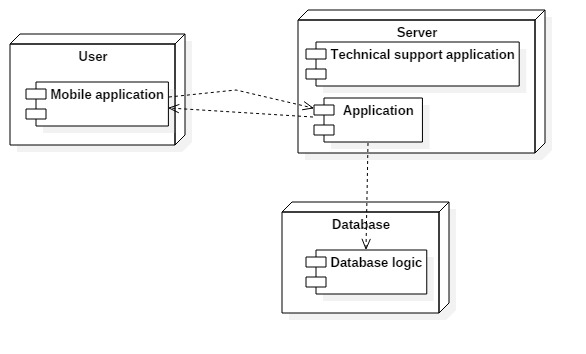
\includegraphics[scale=0.3]{ComponentHighView_241117_1}
	\end{center}
	\caption{High level component diagram}
\end{figure}

From a more detailed point of view, the application on server is made of different components, each one taking care of different functionalities:
\begin{itemize}
	\item Push Gateway: device for sending push notification to the user
	\item MeetingNotifier: is responsible for communication with the user device (notification of upcoming meeting)
	\item Router: handles the incoming data, sorting it to the right controller
	\item ECManager: component containing all the procedures to manage communication with external companies and retrieve all the needed information from them
	\item MeetingBuilder: component that is responsible of creating meetings and breaks and managing the schedule of the user
	\item TripBuilder: component that is responsible of computing trips based on the information retrieved from the ECManager
	\item LoginController: component that controls the registration of clients and their access 
	\item ProfileManager: component that manages the information related to a client (operations such as the setting and change of saved preferences)
	\item InfoProvider: provides access to static information about the system, such as rules and contacts for assistence
\end{itemize}

\begin{figure}[!h]
	\centering
	\begin{center}
		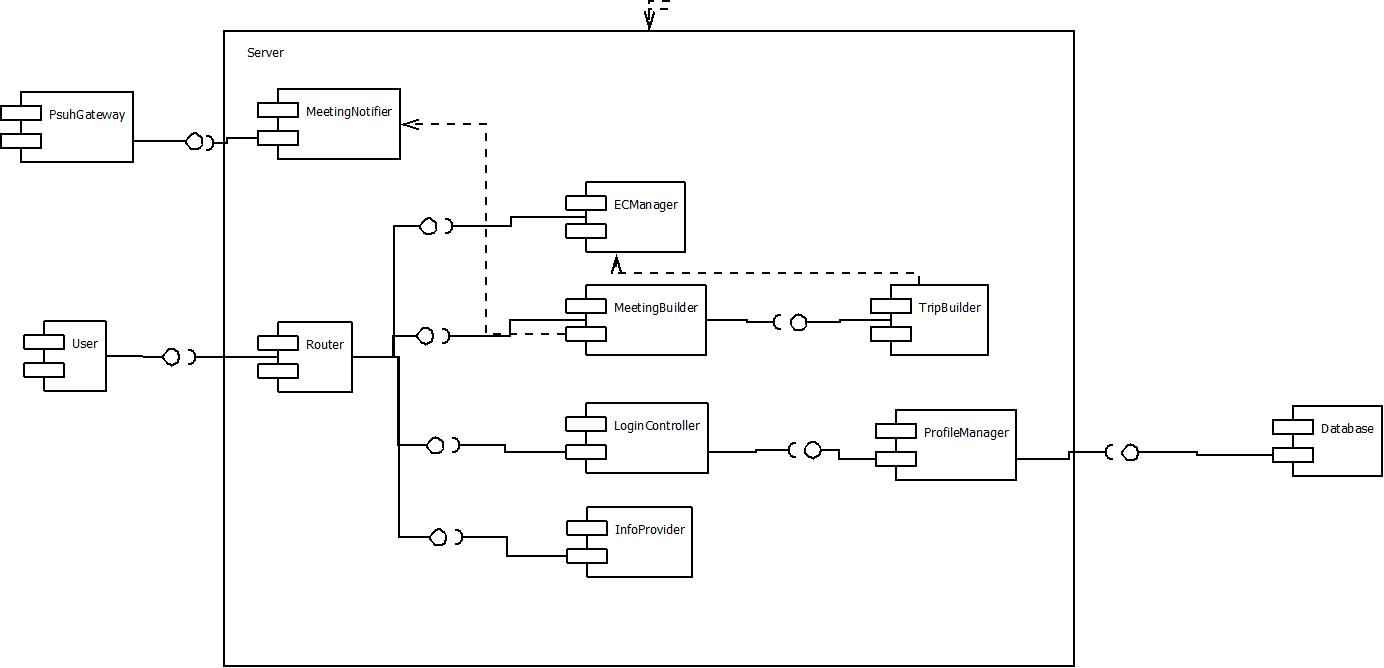
\includegraphics[scale=0.3]{component}
	\end{center}
	\caption{More detailed component diagram}
\end{figure}

\newpage
\subsection{Deployment view}
\begin{figure}[!h]
	\centering
	\begin{center}
		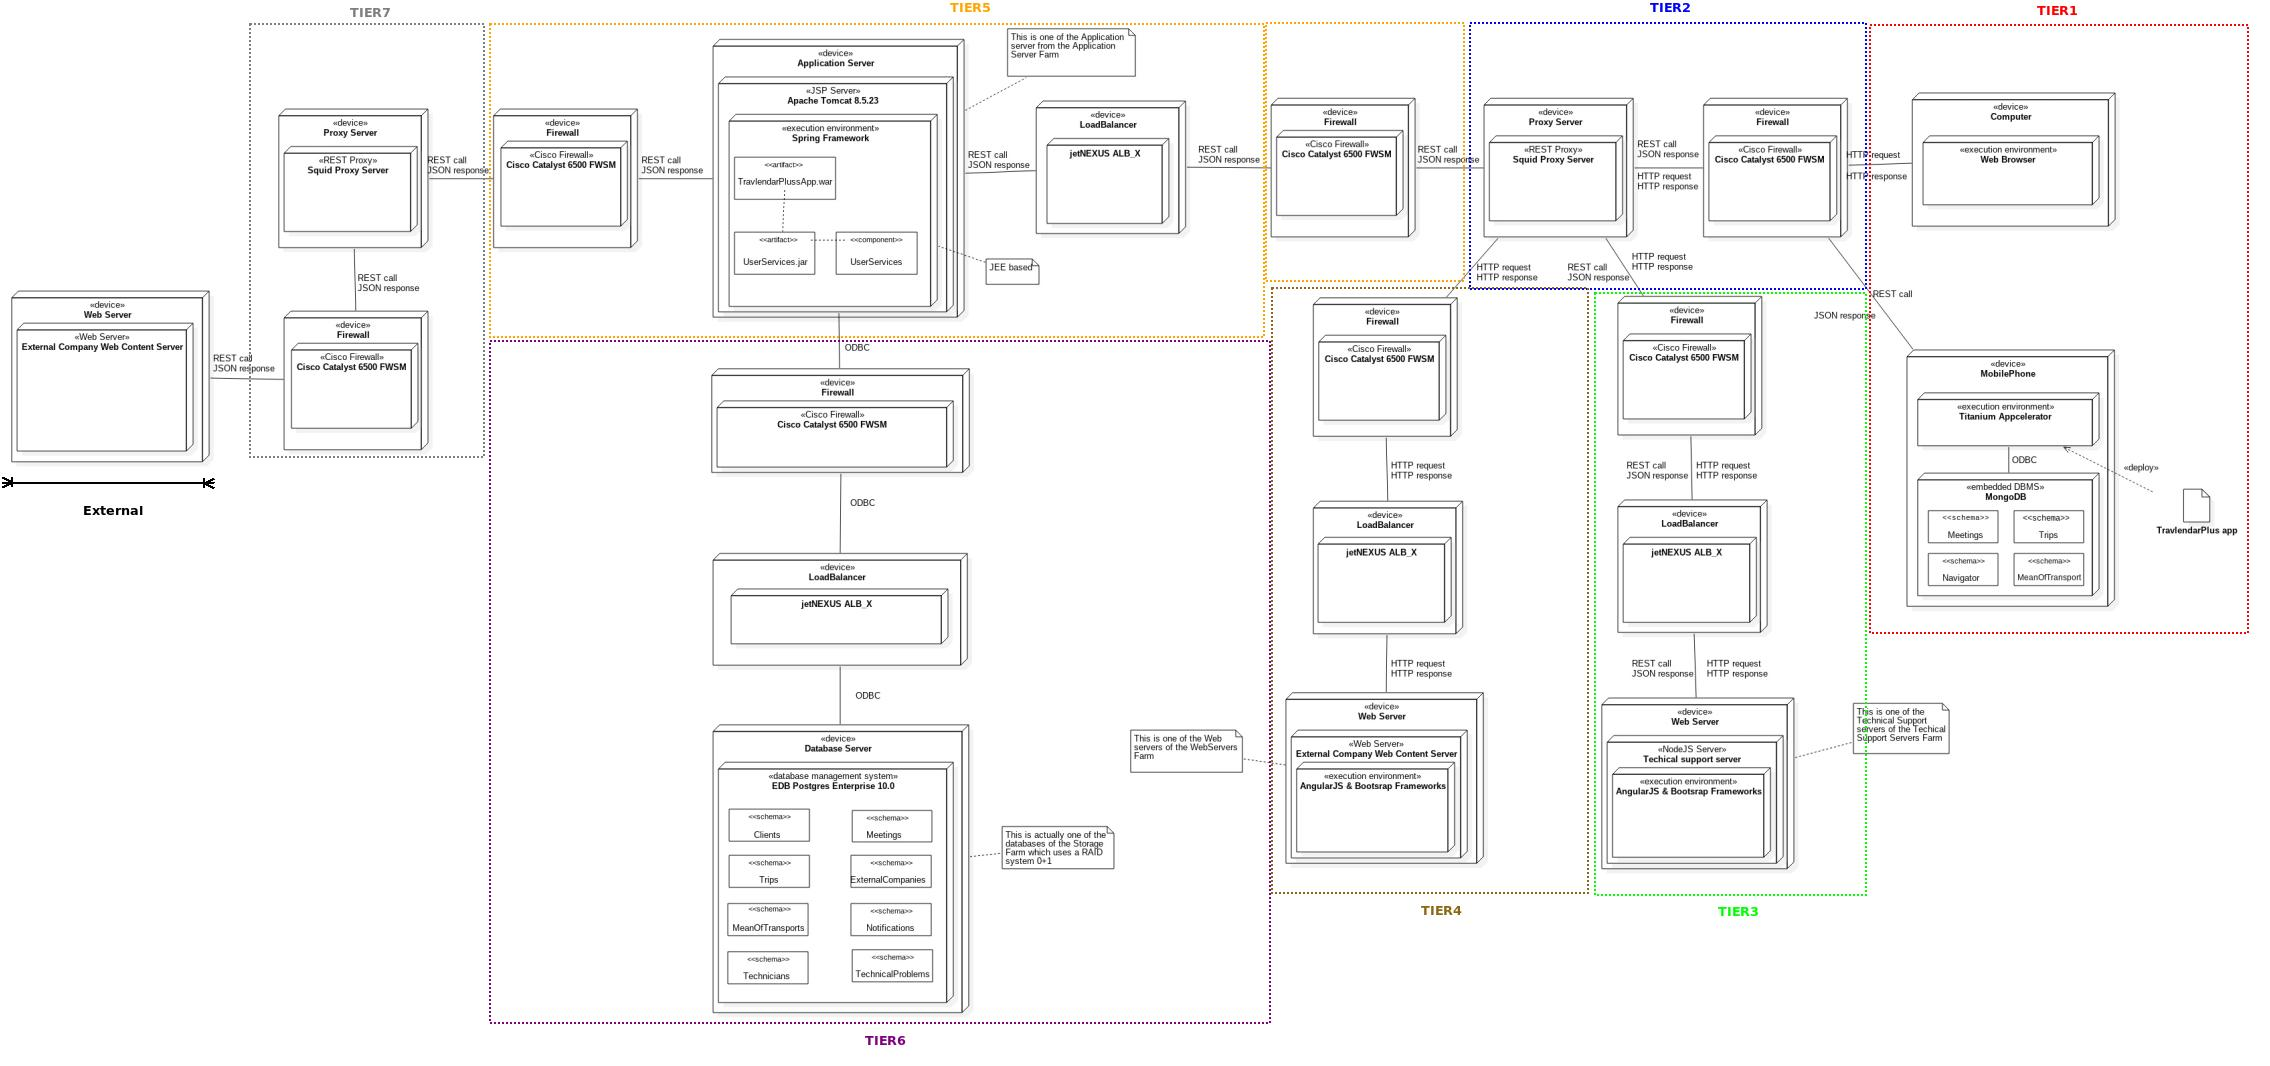
\includegraphics[scale=0.2]{TravlendarPlusDeploymentDiagramTiers_19112017_1}
	\end{center}
       \caption{Deployment diagram}
\end{figure}


\newpage
\subsection{Runtime view}

\subsubsection{Meeting creation}

\begin{figure}[!h]
	\centering
	\begin{center}
		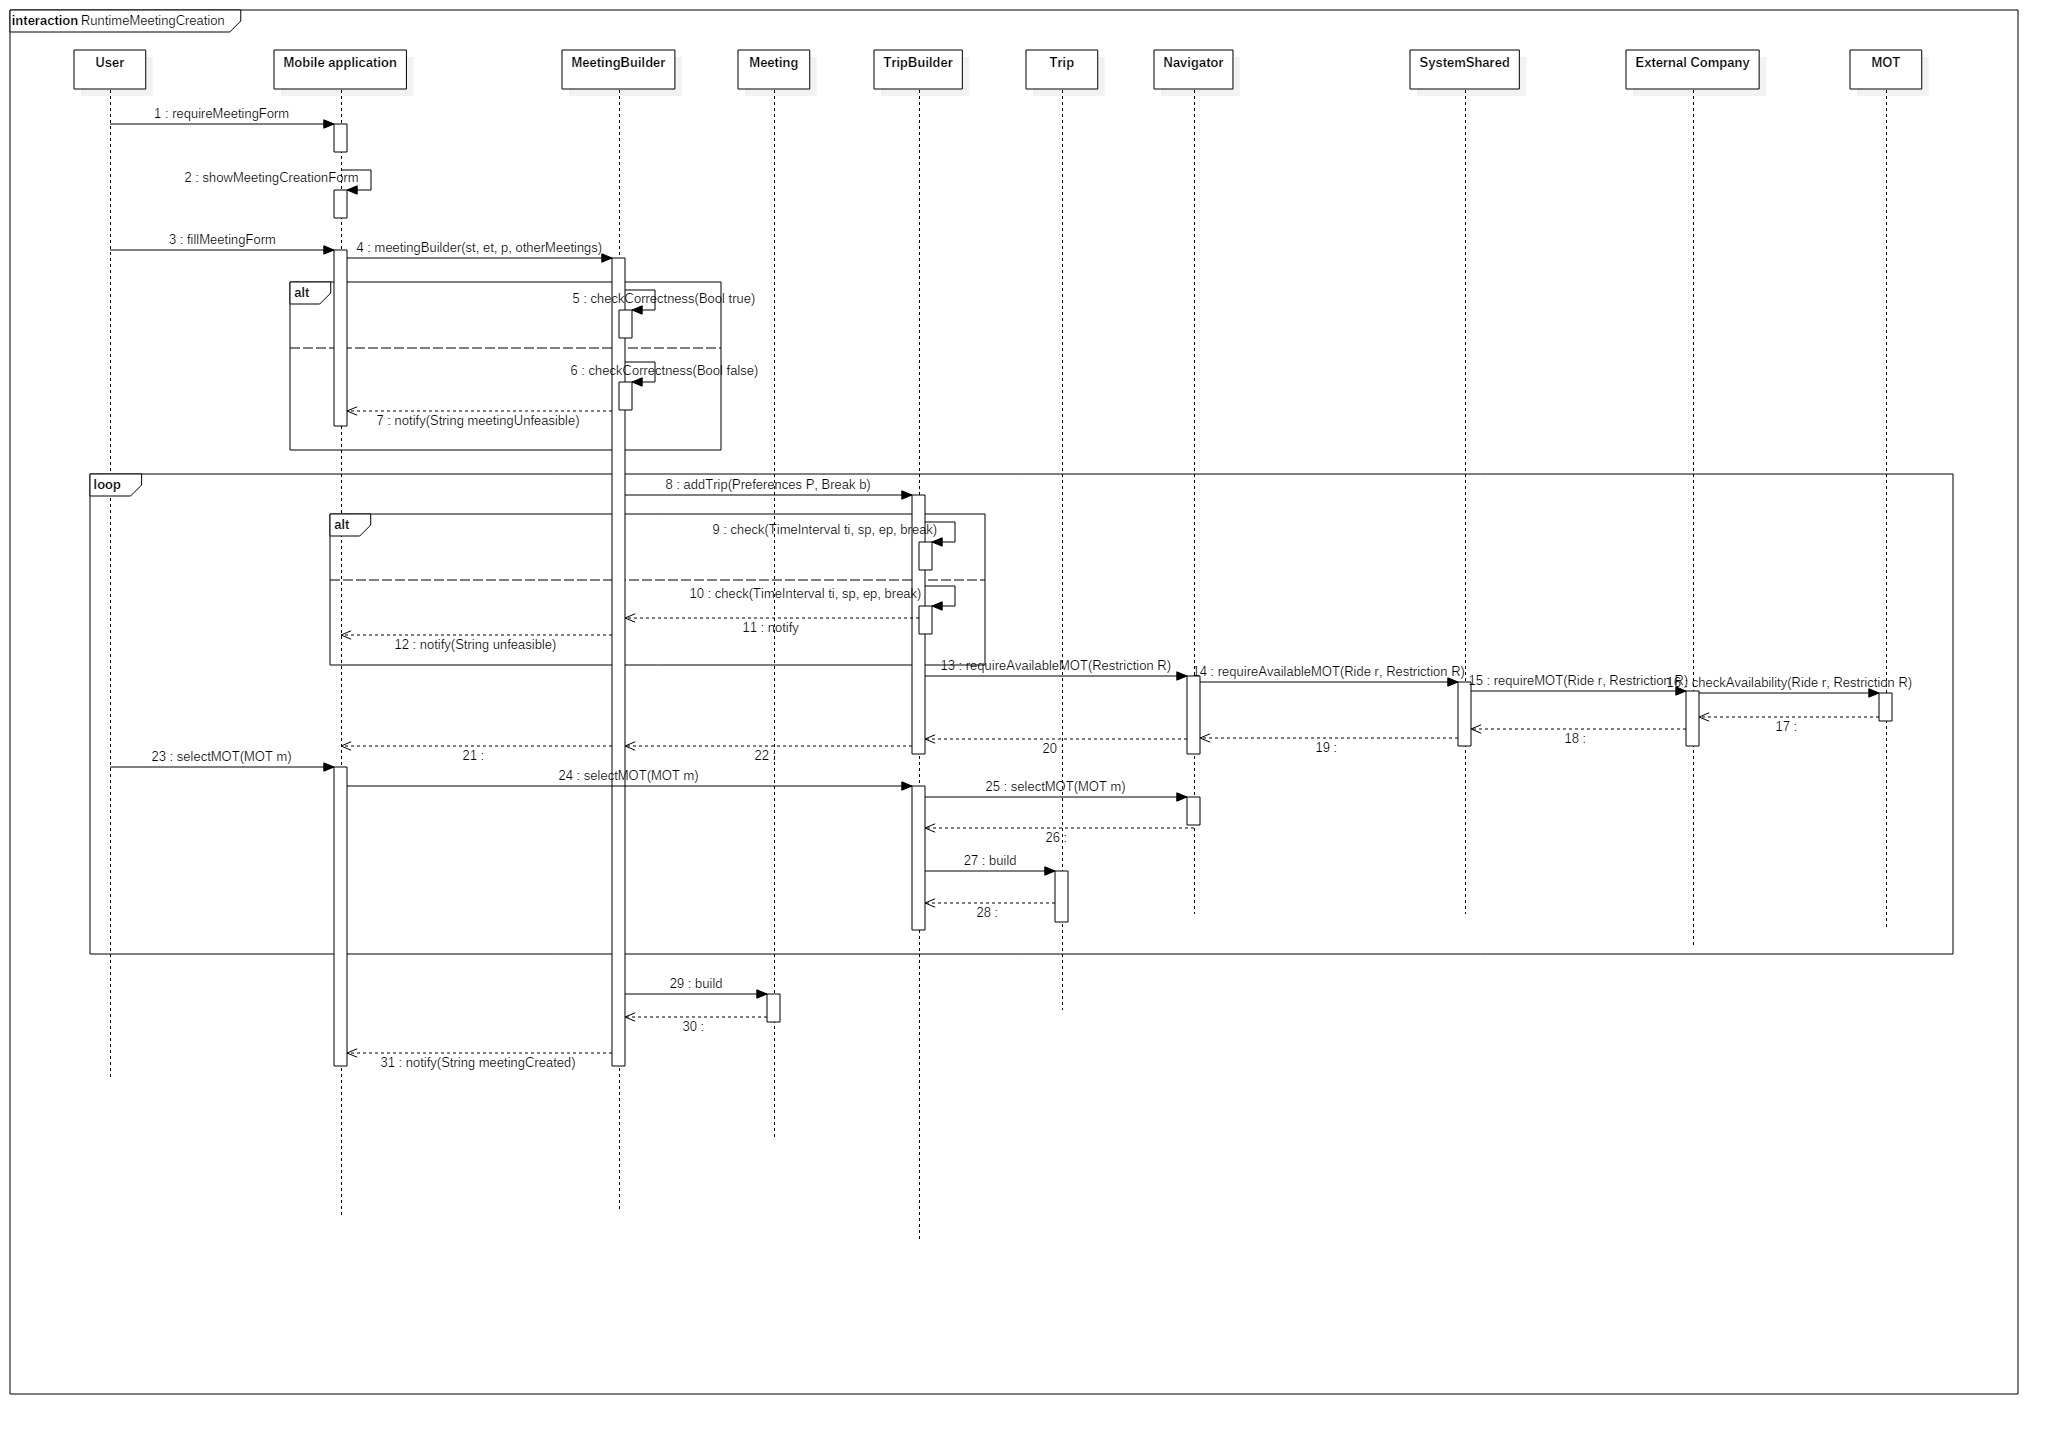
\includegraphics[scale=0.2, angle = 90]{RuntimeMeetingCreation_191117_1}
	\end{center}
	\caption{Runtime sequence diagram of meeting creation}
\end{figure}

This sequence diagram describes the runtime interaction between the components during the creation of a meeting. It refers to use cases 3, 4, 5, 17, 18, 19 and 21 described in section 3.2.2 of the RASD.\\
We illustrated the more general case in which the user is a visitor, that means
an unregistered user: this means that he or she is asked to insert his preferences and constraints (for example deselect unwanted travel means or choice of the most ecological
route) as inputs for the meeting creation. The only difference with a client, or registered user, is that these settings may have been saved, if the user has chosen to,
and they will be searched for in the database.


\subsubsection{Vehicle sharing reservation and ticket purchase}


\begin{figure}[!h]
	\centering
	\begin{center}
		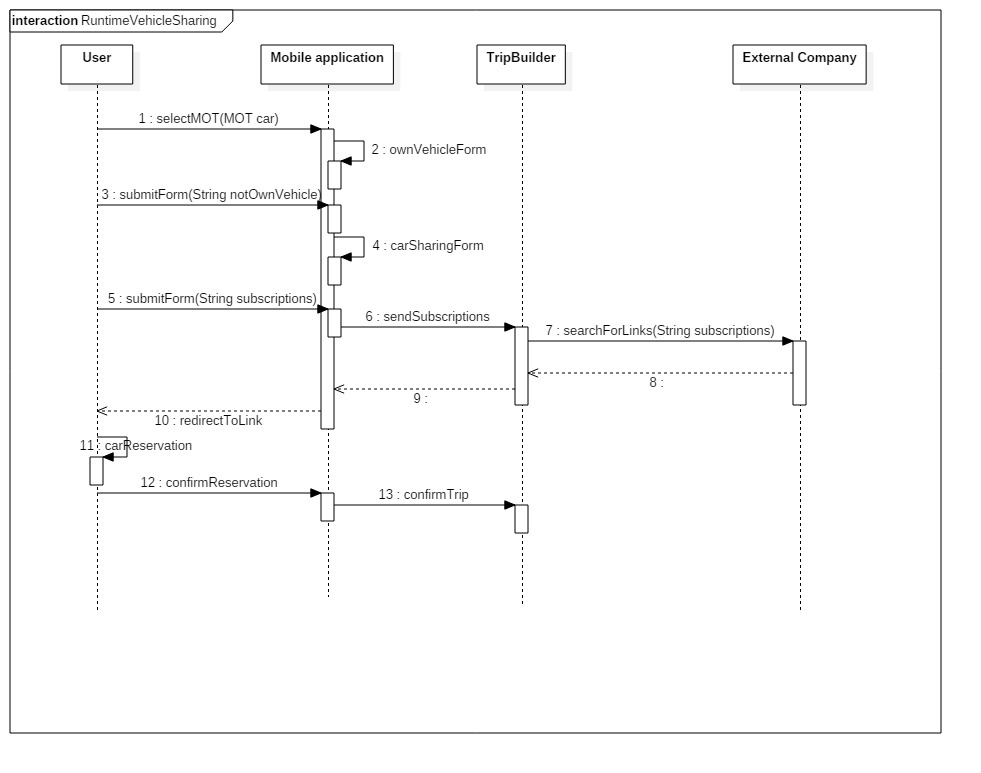
\includegraphics[scale=0.3,]{RuntimeVehicleSharing_191117_1}
	\end{center}
	\caption{Runtime sequence diagram of shared-vehicle reservation}
\end{figure}
\begin{figure}[!h]
	\centering
	\begin{center}
		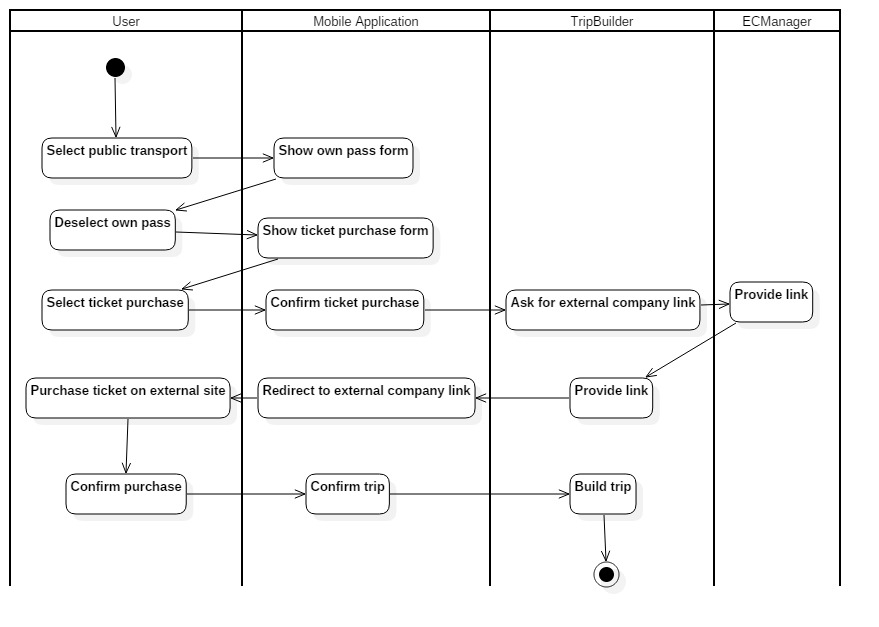
\includegraphics[scale=0.3]{TicketPurchaseActivity_241117_1}
	\end{center}
	\caption{Runtime activity diagram of ticket purchase}
\end{figure}

The top sequence diagram describes the runtime interaction between components during the reservation of a vehicle of a sharing service. A vehicle can be a car, a bike, a 
motorcycle or anything provided by external companies interacting with the system. It refers to use cases 13 and 14 of section 3.2.2 of the RASD.\\
We are in the situation of a meeting creation and the user is selecting the chosen travel means: one of these is a vehicle and the user has not a personal one.
The reservation of a vehicle is perfomed on the external company's website or application; the user is asked for the list of companies for which he or she has a subscription.
Once the reservation is complete, the user confirms the creation of the trip.
A very similar interaction is the purchase of a ticket for a public mean of transport (use case 7 of section 3.2.2 of the RASD), shown in the bottom activity diagram: the user is selecting the travel means during the creation of a meeting and
one of these is a public mean of transport. The user has no personal pass for such transport company. The user is redirected to the company's link, where the purchase
is performed.

\subsection{Component Interfaces}
\subsection{Selected architectural styles and patterns}
Here we describe some of the possible design patterns for the implementation of the system. All the name of classes and inetrfaces refer to the latest version of the class diagram.
\begin{itemize}
	\item Adapter: this pattern has been used to adapt the UserDevice interface to the different operating systems of the users.
	\item Builder
	\item Factory
	\item MVC: this pattern has been overall used to keep separated logic, information and the way they are presented to the user.
	\item Observer: this pattern has been used to manage the notification of problems that may affect travel means, such as strikes or bad weather conditions. The interested classes (MeanOfTransport, Navigator and Trip) are notified when a Notification related to one of such problems changes its status.
	\item Singleton: this pattern has been used for classes that need to be instanciated only a single time; in particular, they are the classes NotificationManager, SystemShared, WindowsPhone, AndroidDevice and iOSDevice
\end{itemize}

\subsection{Other design decisions}

\newpage
\section{Algorithm design}

\newpage
\section{User interface design}
\begin{minipage}[!t]{.5\linewidth}
      \begin{center}
	  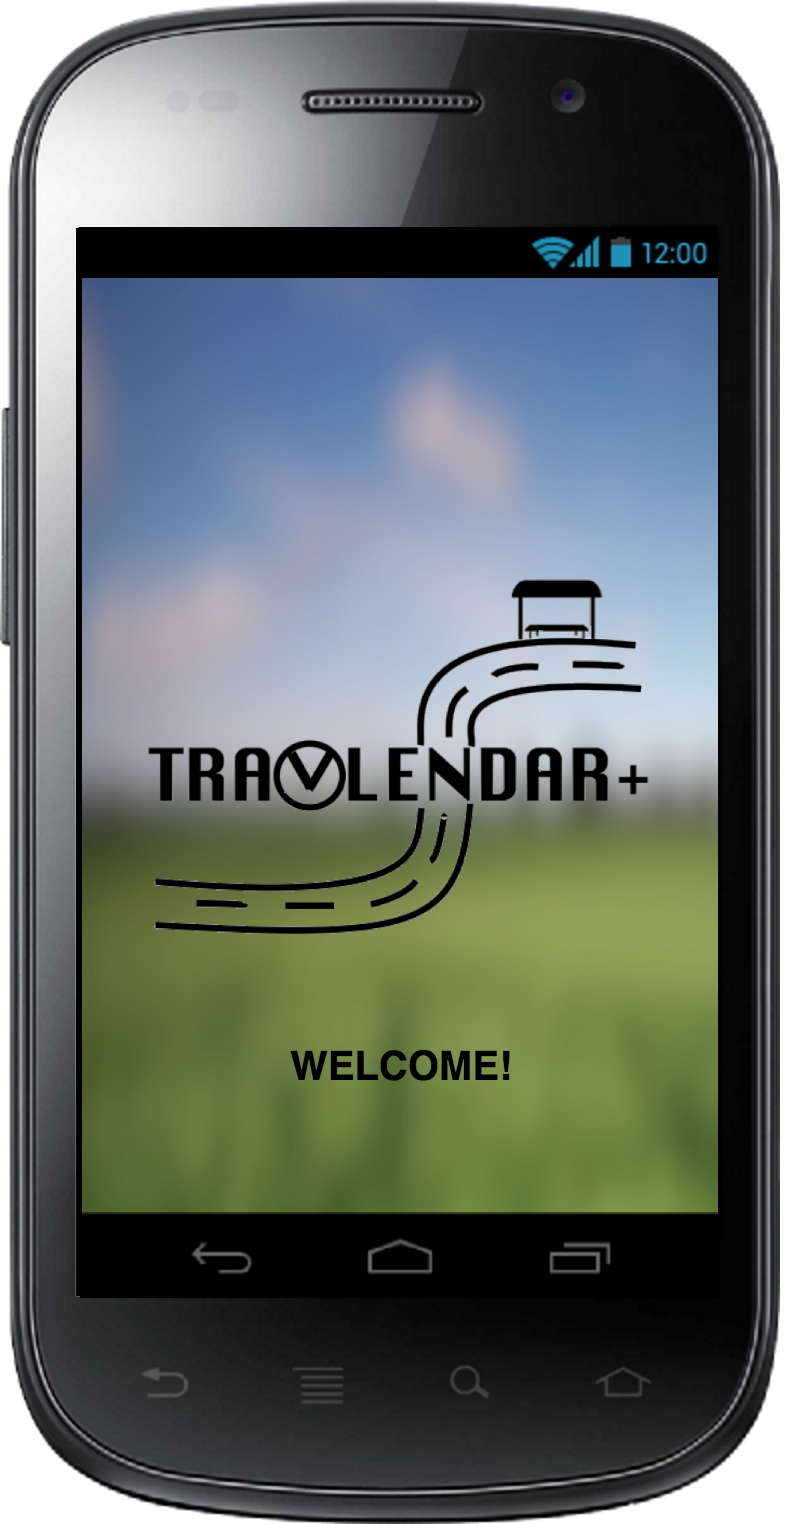
\includegraphics[scale=0.15]{startPage.png}
      \end{center}
\end{minipage}
\begin{minipage}[!t]{.5\linewidth}
	\begin{center}
	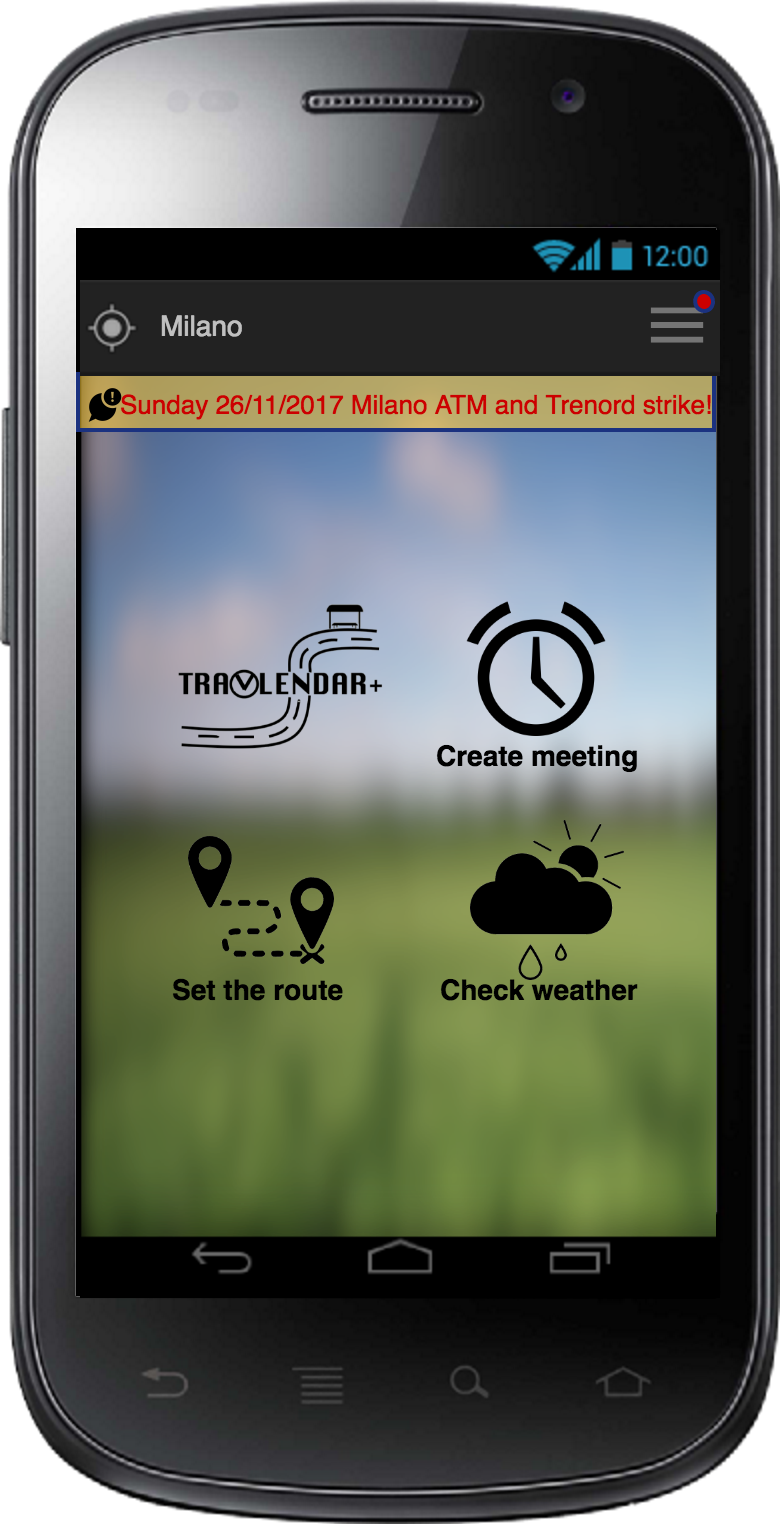
\includegraphics[scale = 0.15]{mainPage.png}
	\end{center}
\end{minipage}
\begin{minipage}[!b]{.5\linewidth}
	\begin{center}
	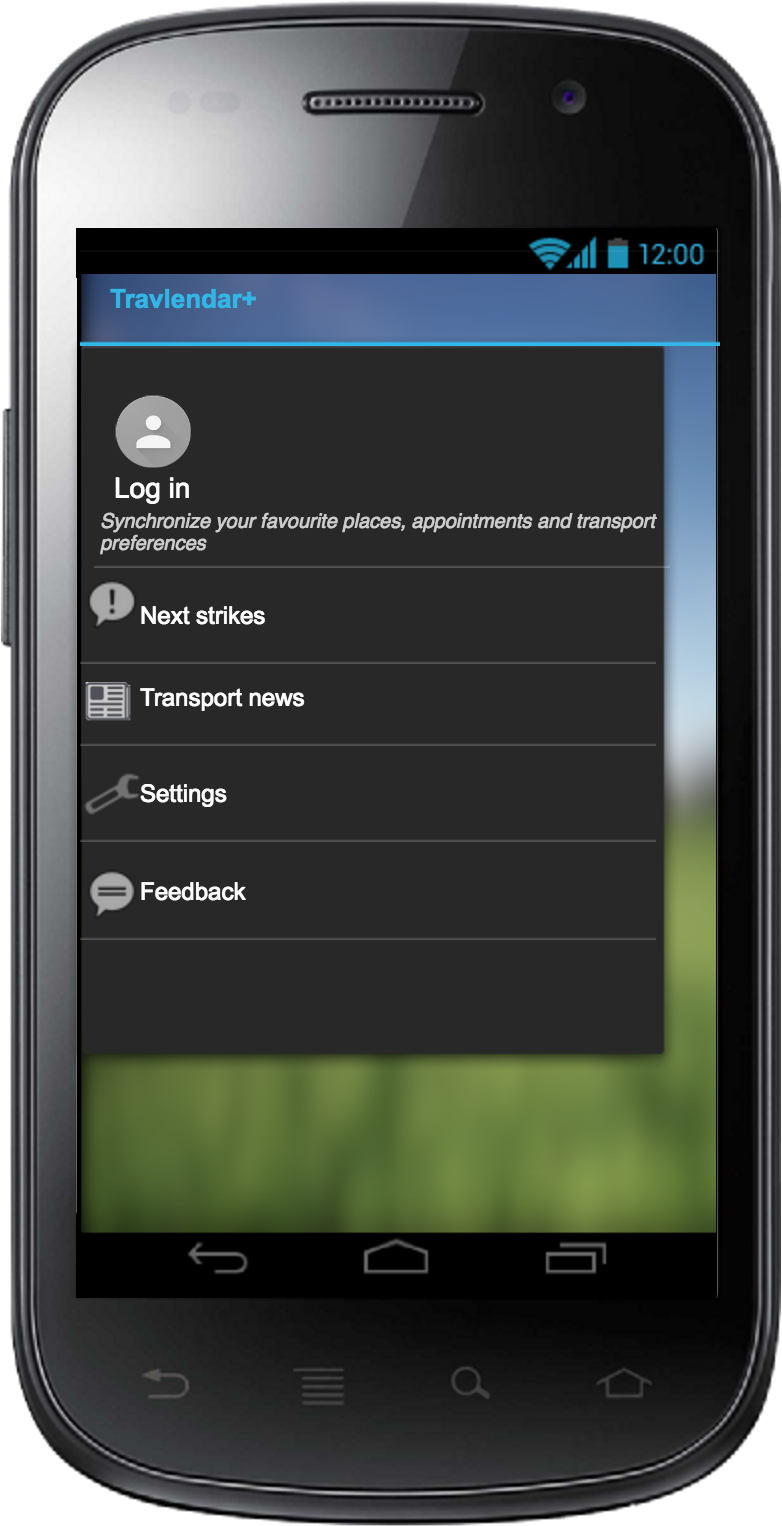
\includegraphics[scale = 0.15]{Menu.png}
	\end{center}
\end{minipage}
\begin{minipage}[!b]{.5\linewidth}
	\begin{center}
	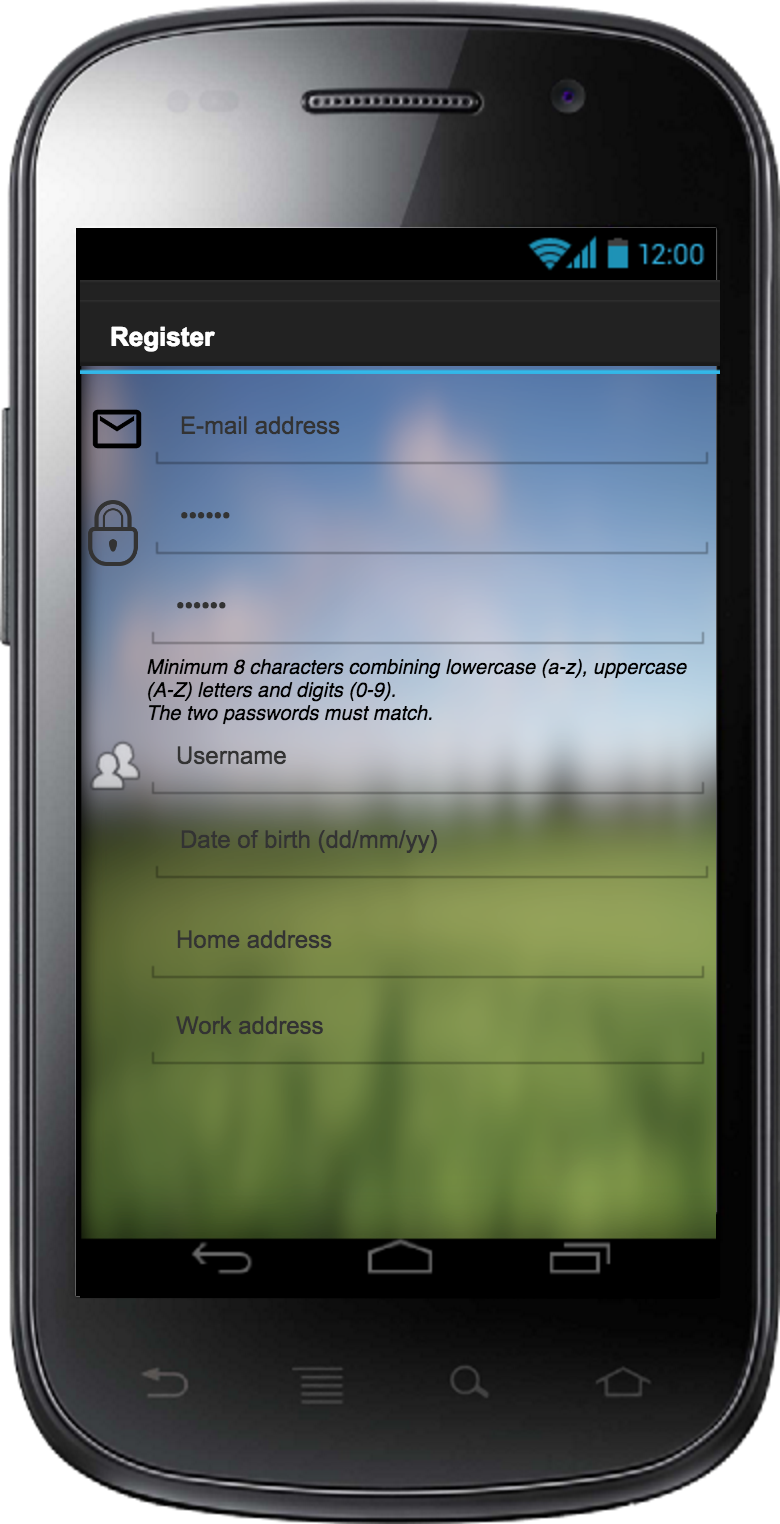
\includegraphics[scale = 0.15]{Registration.png}
	\end{center}
\end{minipage}

\begin{minipage}[!t]{.5\linewidth}
	\begin{center}
		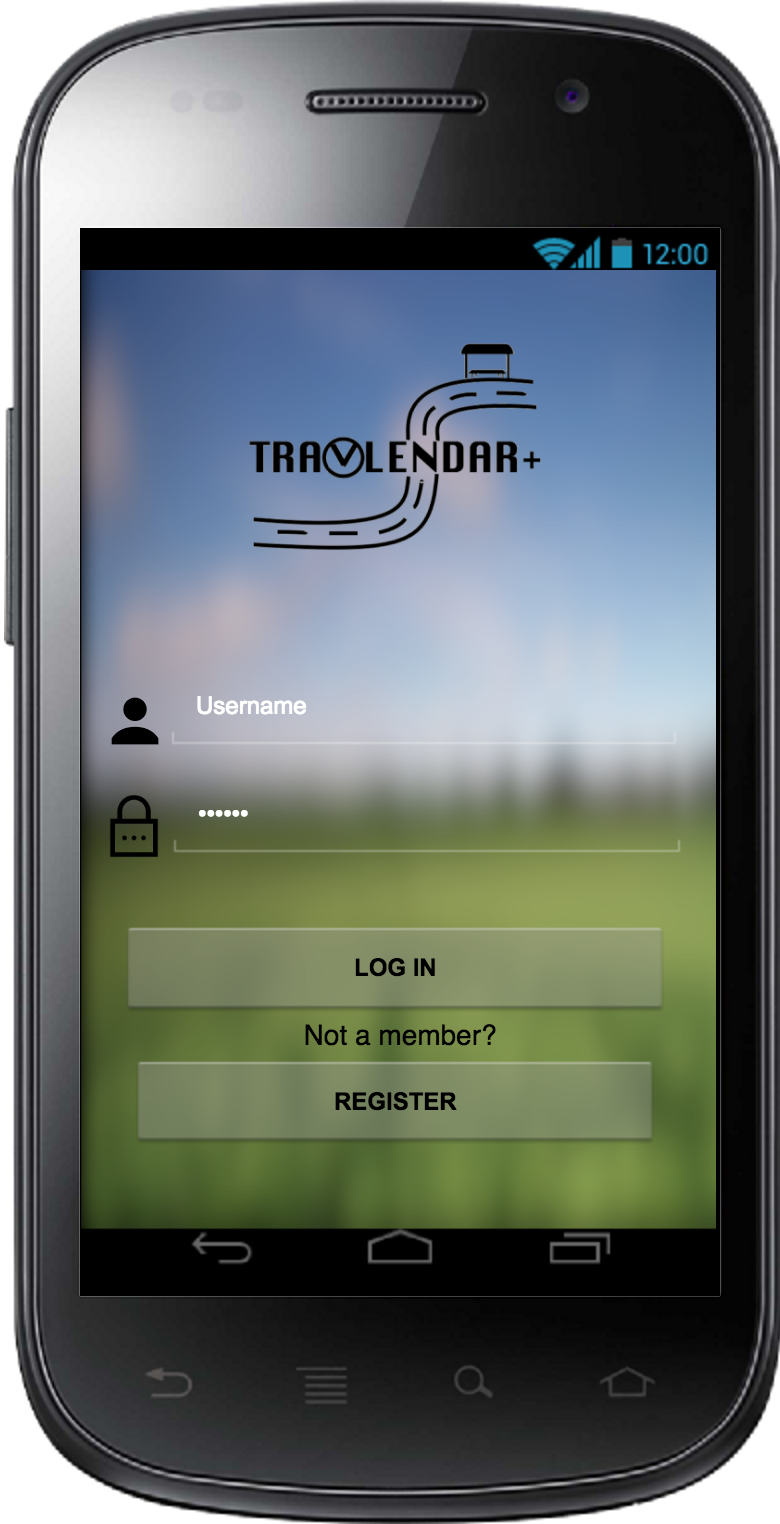
\includegraphics[scale = 0.15]{access.png}
	\end{center}
\end{minipage}

\newpage
\section{Requirements traceability}
In this section we identify which components or functionalities are responsible for the goals and requirements stated in the RASD.

\begin{itemize}
	
	\item (G01): The software should allow the user to register.
	\begin{itemize}
		\item (RE01): The system must allow users to sign in: Mobile application, LoginController
		\item (RE02): The system must allow the client to log in: Mobile Application, LoginController, ProfileManager, Database
		\item (RE03): The system must allow the client to log out: Mobile Application, LoginController
		\item (RE04): The system must allow the client to delete his account: Mobile Application, LoginController, Database
		\item (RE05): The system must provide a high level of security for client's data: LoginController, ProfileManager, Database
	\end{itemize}
	\item (G02): The system allows User to set his/her route inside a city or a region.
	\begin{itemize}
		\item (RE08): The software must allow the user to choose a route: Mobile Application, MeetingBuilder, TripBuilder
		\item (RE09): The software must allow the user to define time constraint to a specific selected route: Mobile Application, MeetingBuilder
	\end{itemize}
	\item (G03): The system allows a User to choose a kind of transport among pre-defined travel means according to his/her preferences
	\begin{itemize}
		\item (RE10): For each path the software must provide all the available means of transport that can be used, according to the software interfaces: Mobile Application, TripBuilder, ECManager
		\item (RE11): The software must allow the user to select vehicles that he/she wants to use for the route: Mobile Application, MeetingBuilder
		\item (RE15): If a route is not possible because the selected travel mean is not allowed to pass a specific place, the application must deny that option and notify the user: Mobile Application, ECManager, TripBuilder, MeetingNotifier, PushGateway
	\end{itemize}
	\item (G04): The system allows a User to reserve a range of time for breaks.
	\begin{itemize}
		\item (RE12): The software must require the estimated time for a break: Mobile Application, MeetingBuilder 
		\item (RE16): If a route is not possible because breaks requires too much time, the application must deny that option and notify the user: Mobile Application, MeetingBuilder
		\item (RE20): If a break runs out the selected time the application must notify the user: Mobile Application, MeetingBuilder
	\end{itemize}
	\item (G05): The system must communicate to the user that a path (selected by this one) is not reachable or it's out of time.
	\begin{itemize}
		\item (RE14): If a route is not possible because the required time to reach the destination is not enough, the application must deny that option and notify the user: Mobile Application, MeetingBuilder, TripBuilder
	\end{itemize}
	\item (G06): The system must provide all the possible path that can be taken by a user, according to his/her needs.
	\begin{itemize}
		\item (RE17): The software must provide a User all the available solutions, according to his/her selected preferences, to get from one place to another: Mobile Application, TripBuilder
	\end{itemize}
	\item (G07): The system must provide firstly the most optimized and suitable solution, according to the user preferences.
	\begin{itemize}
		\item (RE19): The application should provide, as first option, the optimal solution according to the users's preferences about minimizing carbon footprint: Mobile Application,  MeetingBuilder, TripBuilder
	\end{itemize}
	\item (G08): The system must provide information about problems/strikes for all the travel means  included in the software.
	\begin{itemize}
		\item (RE18): The software must inform the user about problems with using some transport (strikes , road damages, rain and so on) for which the usability is not guaranteed: Mobile Application, ECManager, TripBuilder, MeetingNotifier
		\item (RE21): The application should avoid to make the user pass through dangerous zones of a city or a region: TripBuilder, ECManager
		\item (RE22): If the user has to pass through a dangeousr zone, the application must inform him/her: Mobile Application, TripBuilder, ECManager, MeetingNotifier
	\end{itemize}
	\item (G09): The system must provide a user the information about weather conditions during his/her planned route: Mobile Application, MeetingNotifier
	\item (G10): The system must provide a way to permit a user to buy a ticket for public transports.
	\begin{itemize}
		\item (RE07): The software must interface with all major public transport companies that provide API: ECManager
	\end{itemize}
	\item (G11): The system must provide the nearest location of a bike provided by a pre-defined bike sharing service provider: TripBuilder, ECManager
	\item (G12): The system must provide the nearest location of a car provided by a pre-defined car sharing service provider: TripBuilder, ECManager
	\item (G13): The system must avoid overlaps in user's scheduled travels.
	\begin{itemize}
		\item (RE13): If a route is not possible because of overlaps with other journeys, the application must deny that option and notify the user: MeetingBuilder
	\end{itemize}
	\item (G14): The system must allow the user to create meetings with different priority.
	\begin{itemize}
		\item (RE23):  The software must require the estimated time for a meeting: Mobile Application, MeetingBuilder
		\item (RE24): For each meeting, the system should ask the user to define its priority (1-business, 2-appointment, 3-with friends, 4-personal): Mobile Application, MeetingBuilder
	\end{itemize}
	\item (G15): The system must inform the user about upcoming meetings.
	\begin{itemize}
		\item (RE25): The system should warn about upcoming meetings twenty minutes before: MeetingNotifier, PushGateway
	\end{itemize}
	\item (G16): The system must allow the user to change the part of the path during his/her trip: Mobile Application, MeetingBuilder, TripBuilder
	\item (G17): The system must provide an alternative path in case of problems along the selected one: Mobile Application, TripBuilder, ECManager
	\item (G18): The software should show a user, if possible, the combination of travel means that minimize the carbon footprint, according to the selected path and the required time: Mobile Application, TripBuilder, MeetingBuilder
	
\end{itemize} 

\newpage
\section{Implementation, integration and test plan}

\subsection{Integration and test}

\subsubsection{Entry criteria}
In order to begin the integration and test phase, the following assumptions must be valid:

\begin{itemize}
	\item The RASD and the previous sections of DD must be complete and correct
	\item The database must be complete, configured and operating
	\item The APIs of external companies collaborating with the system must be usable
	\item The main functionalities of the server's components have been implemented and unit tested
\end{itemize}

\subsubsection{Integration testing strategy}
We plan to test and integrate the components incrementally, as soon as they have been implemented and unit tested. As for the implementation, we plan to adopt a mainly bottom up strategy, although slight changes to this approach can be adopted if nit doesn't have to be strictly followed and small changes to this approach can be made, when needed.
We also plan to adopt a critical module approach, testing first the modules which perform the main functionalities of the system.

\subsubsection{Sequence of integration}
As stated in the previous subsection, we will test the main functionalities of the system as soon as possible, which are the creation of meetings and the computation of trips. These are performed by the MeetingBuilder and the TripBuilder. However, the TripBuilder needs to retrieve the information from the collaborating external companies and the communication with those is managed by the ECManager. Assuming that the ECManager is fully working and able to provide reliable information from the external companies, the first two elements to be integrated are the ECManager and the TripBuilder, followed by the TripBuilder and the MeetingBuilder.\\
In parallel, the integration of the PushGateway and the MeetingNotifier can be performed and, once the MeetingBuilder is integrated with the previous components, between MeetingNotifier and MeetingBuilder.\\
The login and preference savings are functionalities we are thinking to add in a second phase: in fact, they are not strictly required for the functioning of the system, but we think they may be useful for security related issues and for a better user's fidelization. Therefore they don't need to be integrated at once and we preferred to give precedence to the components stated so far.\\
The integration of these components with the router will then be performed and after this the server can be considered fully tested. We will then proceed with the integration of the database and, finally, the user.

\newpage
\section{Effort spent}
\subsection{Bolshakova Liubov}
\begin{itemize}
	\item 
\end{itemize}
\subsection{Campagnoli Chiara}
\begin{itemize}
	\item 
\end{itemize}
\subsection{Lagni Luca}
\begin{itemize}
	\item 
\end{itemize}

%\newpage
%\section{References}
	
\end{document}